

%%%%%%%%%%%%%%%%%%%%%%%%%%%%%%%%%%%%%%%%%%%%%%%%%%%%%%%%%%%%%%%%%%%%%%%%%%%%%%%%
%%%%%%%%%%%%%%%%%%%%%%%%%%%%%%%%%%%%%%%%%%%%%%%%%%%%%%%%%%%%%%%%%%%%%%%%%%%%%%%%
%%%%%%%%%%%%%%%%%%%%%%%%%%%%%%%%%%%%%%%%%%%%%%%%%%%%%%%%%%%%%%%%%%%%%%%%%%%%%%%%
\section{Regularização}

\index{Regularização}


A regularização é o processo pelo qual um problema \illposed~é 
aproximado por uma família vizinha de problemas catalogados como \wellposed~\cite[pp. 49]{engl2000regularization},
para realizar esta aproximação, nova informação  é adicionada ao problema.
Por exemplo, podemos aplicar a regularização agregando uma função objetivo para criar um problema de otimização
a partir do problema \illposed.

\begin{description}
\item[Problema direto:] Considere um sistema representado pelo seguinte problema direto,
\begin{equation}\label{eq:regularization:1}
\MATRIX{A}\VECTOR{x}=\VECTOR{y},
\end{equation}
onde a resposta vector $\VECTOR{y}\in \mathbb{R}^M$ é obtida logo de introduzir o estimulo $\VECTOR{x}\in \mathbb{R}^N$,
sendo $\MATRIX{A}:\mathbb{R}^N \rightarrow \mathbb{R}^M$ uma matriz operador linear.

\item[Problema inverso:] O problema inverso para o sistema da Eq. (\ref{eq:regularization:1}), é
achar o vetor de entrada $\VECTOR{x}$, que cumpra  a Eq. (\ref{eq:regularization:2})
onde $\VECTOR{y}_{\delta}$ é um vetor com amostras ruidosas de $\VECTOR{y}$,
e $0\leq||\VECTOR{y}-\VECTOR{y}_{\delta}||^2\leq \delta^2$,
\begin{equation}\label{eq:regularization:2}
\MATRIX{A}\VECTOR{x}=\VECTOR{y}_{\delta}.
\end{equation}
Se o sistema da Eq. (\ref{eq:regularization:2}) estiver \wellposed,
então a solução única é $\VECTOR{x}=\MATRIX{A}^{-1}\VECTOR{y}_{\delta}$ se $M=N$,
ou $\VECTOR{x}=\left\{\MATRIX{A}^{\transpose}\MATRIX{A}\right\}^{-1}\MATRIX{A}^{\transpose}\VECTOR{y}_{\delta}$ se $M\neq N$.

Porém, se o problema da Eq. (\ref{eq:regularization:2}) estiver \illposed,
então não é possível obter uma solução única.\\
\end{description}

Assim, para resolver o problema inverso \illposed~temos que aplicar uma regularização;
é dizer; nova informação tem que ser agregada;
porém, na regularização da Eq. (\ref{eq:regularization:2}) podemos ter abordagens diferentes dependendo 
se não existe solução ou se existem múltiplas soluções. 
%%%%%%%%%%%%%%%%%%%%%%%%%%%%%%%%%%%%%%%%%%%%%%%%%%%%%%%%%%%%%%%%%%%%%%%%%%%%%%%%
\subsection{Quando um problema \illposed~não tem solução}
Se sabemos que a Eq. (\ref{eq:regularization:2}) não tem solução, como no Exemplo \ref{ex:IllPosedNoSolutions}, 
uma forma de regularizar este problema, consiste em aceitar a impossibilidade da igualdade na equação, 
e transformar esta numa função de custo $e(\VECTOR{x})$, usando o critério de procurar o mínimo erro quadrático,
\begin{equation}\label{eq:regularization:3}
e(\VECTOR{x})=||\MATRIX{A}\VECTOR{x}-\VECTOR{y}_{\delta}||^2,
\end{equation}
de modo que no melhor dos casos o mínimo $e(\VECTOR{x})$ tomará o valor zero, 
porém também aceitaremos uma solução $\VECTOR{x}$ que produz um mínimo $e(\VECTOR{x})$  maior a zero.
%Na Seção \ref{sec:minAxbCAxb} veremos mais a detalhe como resolver o problema de minimização proposto na Eq. (\ref{eq:regularization:3}).
\begin{SolutionT}[Relativa ao Exemplo \ref{ex:IllPosedNoSolutions}:]
Como é descrito na Seção \ref{sec:minAxbCAxb}, para resolver um problema de minimização como o proposto na Eq. (\ref{eq:regularization:3}),
podemos usar o Teorema \ref{theo:minAxbCAxb}, de modo que o vetor $\VECTOR{x}=\VECTOR{\hat{x}}$ que minimiza $e(\VECTOR{x})$
é igual a
\begin{equation}\label{eq:regularization:3b}
\VECTOR{\hat{x}} =
\left[ \MATRIX{A}^{\transpose} \MATRIX{A} \right]^{-1}\MATRIX{A}^{\transpose}\VECTOR{y}_{\delta}
=
\begin{bmatrix}
0.50000 \\
1.83333
\end{bmatrix}
\qquad \leftarrow \qquad
\MATRIX{A}=
\begin{bmatrix}
1 & 1\\
2 & 1\\
0 & 1
\end{bmatrix},
\qquad
\VECTOR{y}_{\delta}=
\begin{bmatrix}
2\\
3\\
2
\end{bmatrix},
\end{equation}
como é visto na Figura \ref{fig:ex:IllPosedNoSolutions:a}, 
onde é desenhada a superfície $e(\VECTOR{x})$ e o ponto mínimo $\VECTOR{\hat{x}}$.
Se analisamos $\VECTOR{\hat{x}}$ em relação à Eq. (\ref{eq:regularization:2}),
observaremos que este vetor de entrada produz uma resposta $\VECTOR{\hat{y}}$ que é diferente de $\VECTOR{y}_{\delta}$,
\begin{equation}
\MATRIX{A}\VECTOR{\hat{x}}= \VECTOR{\hat{y}} =
\begin{bmatrix}
2.3333\\
2.8333\\
1.8333
\end{bmatrix}
\neq \VECTOR{y}_{\delta}.
\end{equation}
Na Figura \ref{fig:ex:IllPosedNoSolutions:b} podemos ver graficamente a relação entre os pontos (vetores)
$\VECTOR{\hat{y}}$ e $\VECTOR{y}_{\delta}$,
onde o ponto $\VECTOR{\hat{y}}$ encontra-se dentro do plano $\MATRIX{A}\VECTOR{x}$,
porém o ponto $\VECTOR{y}_{\delta}$ não pertence a esse plano, 
motivo pelo qual era impossível achar uma solução à Eq. (\ref{eq:regularization:2});
nesse sentido, a regularização do problema nos habilitou a achar $\VECTOR{\hat{y}}$,
que é o ponto no plano  $\MATRIX{A}\VECTOR{x}$ mais próximo a $\VECTOR{y}_{\delta}$;
é dizer, este é o ponto de interseção do plano e uma linha perpendicular que parte de $\VECTOR{y}_{\delta}$.
\end{SolutionT}

\begin{figure}[h!]
     \centering
     \begin{subfigure}[b]{0.475\textwidth}
         \centering
         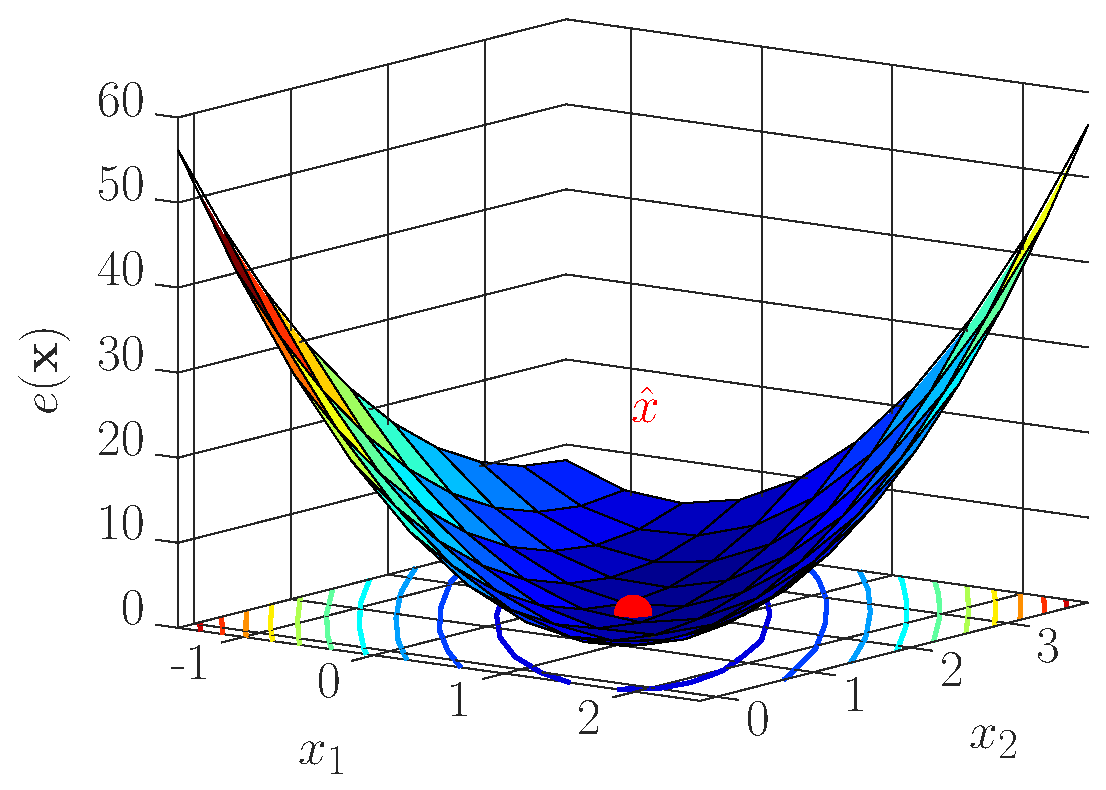
\includegraphics[width=0.98\textwidth]{chapters/notacao/mfiles/illpossed1/surfcex.eps}
         \caption{Superfície $e(\VECTOR{x})$ e o ponto $\VECTOR{\hat{x}}$. }
         \label{fig:ex:IllPosedNoSolutions:a}
     \end{subfigure}
     \hfill
     \begin{subfigure}[b]{0.475\textwidth}
         \centering
         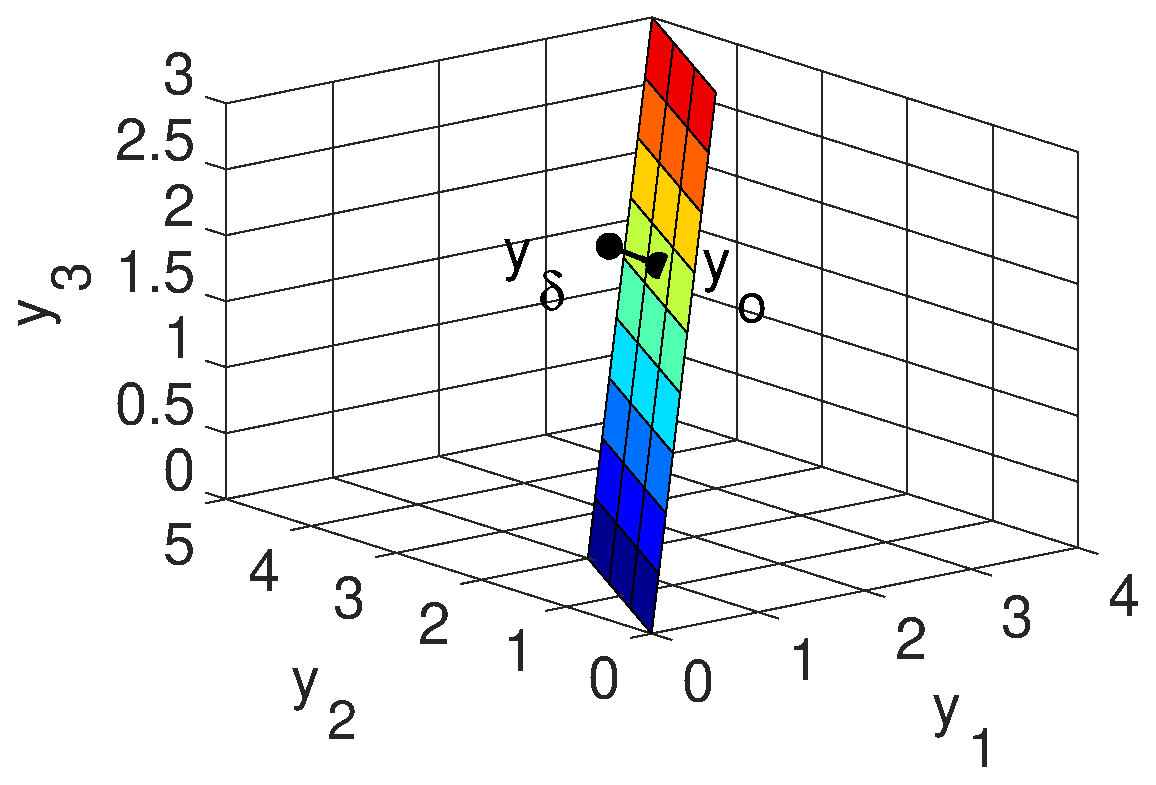
\includegraphics[width=0.98\textwidth]{chapters/notacao/mfiles/illpossed1/surfcax.eps}
         \caption{Plano $\MATRIX{A}\VECTOR{x}=\VECTOR{y}$ e os pontos $\VECTOR{y}_{\delta}$ e $\VECTOR{\hat{y}}$.}
         \label{fig:ex:IllPosedNoSolutions:b}
     \end{subfigure}
        \caption{Resposta gráfica do Exemplo \ref{ex:IllPosedNoSolutions}. }
        \label{fig:ex:IllPosedNoSolutions}
\end{figure}

%%%%%%%%%%%%%%%%%%%%%%%%%%%%%%%%%%%%%%%%%%%%%%%%%%%%%%%%%%%%%%%%%%%%%%%%%%%%%%%%
\subsection{Quando um problema \illposed~ tem muitas soluções}
Quando a Eq. (\ref{eq:regularization:2}) tem múltiplas soluções, 
não é possível regularizar o problema com uma função de custo da forma 
$||\MATRIX{A}\VECTOR{x}-\VECTOR{y}_{\delta}||^2$,
pois o problema nunca foi achar um ponto $\VECTOR{x}$ que cumpra a Eq. (\ref{eq:regularization:2}), 
e sim ter um critério para escolher uma resposta $\VECTOR{x}=\VECTOR{\hat{x}}$ entre os muitos valores que pode tomar este ponto;
assim, se abordamos o problema da Eq. (\ref{eq:regularization:2}) tentando minimizar $||\MATRIX{A}\VECTOR{x}-\VECTOR{y}_{\delta}||^2$,
com uma resposta $\VECTOR{\hat{x}} = \left[ \MATRIX{A}^{\transpose} \MATRIX{A} \right]^{-1}\MATRIX{A}^{\transpose}\VECTOR{y}_{\delta}$
como na Eq. (\ref{eq:regularization:3b}),
perceberemos que a matriz $\MATRIX{A}^{\transpose}\MATRIX{A}$ não tem inversa,
pelo que a resposta não pode ser calculada;
pois se a matriz fosse invertível teríamos uma única resposta e não saberíamos
qual foi o critério para escolher esta em particular.

Para abordar problemas deste tipo; é dizer com multiplas soluções
como o apresentado no Exemplo \ref{ex:IllPosedMultiplaSolutions}, 
poderíamos propor uma regularização baseada na minimização
da função 
\begin{equation}\label{eq:regularization:4}
e(\VECTOR{x})=||\MATRIX{A}\VECTOR{x}-\VECTOR{y}_{\delta}||^2+||\VECTOR{x}||^2,
\end{equation}
que nos ajuda a procurar uma solução que penaliza a resposta $\VECTOR{x}=\VECTOR{\hat{x}}$ da função de custo $e(\VECTOR{x})$, 
quanto maior seja o valor $||\VECTOR{x}||^2$;
é dizer, a resposta é de menor interesse quanto mais longe esteja do ponto $\VECTOR{0}$.

%Na Seção \ref{sec:minAxbCAxbplusalphaxqD} veremos mais a detalhe como resolver o problema de minimização proposto na Eq. (\ref{eq:regularization:4}).
\begin{SolutionT}[Relativa ao Exemplo \ref{ex:IllPosedMultiplaSolutions}:]
\label{sol:IllPosedMultiplaSolutions}
Como é descrito na Seção \ref{sec:minAxbCAxbplusalphaxqD}, 
para resolver um problema de minimização como o proposto na Eq. (\ref{eq:regularization:4}),
podemos usar o Teorema \ref{theo:minAxbCAxbplusalphaxqD}, 
de modo que o vetor $\VECTOR{x}=\VECTOR{\hat{x}}$ que minimiza $e(\VECTOR{x})$
é igual a
\begin{equation}\label{eq:regularization:4b}
\VECTOR{\hat{x}} =
\left[ \MATRIX{A}^{\transpose}\MATRIX{A} +\MATRIX{I}\right]^{-1} \MATRIX{A}^{\transpose} \VECTOR{y}_{\delta}
=
\begin{bmatrix}
0.85714\\
0.85714
\end{bmatrix}
\qquad \leftarrow \qquad
\MATRIX{A}=
\begin{bmatrix}
1 & 1\\
1 & 1\\
1 & 1
\end{bmatrix}
\qquad
\VECTOR{y}_{\delta}=
\begin{bmatrix}
2\\
2\\
2
\end{bmatrix}.
\end{equation}
É importante lembrar que $\VECTOR{x}=\VECTOR{\hat{x}}$ minimiza a função $e(\VECTOR{x})$ e não
a função $||\MATRIX{A}\VECTOR{x}-\VECTOR{y}_{\delta}||^2$,
pelo que como podemos ver na Figura \ref{fig:ex:IllPosedMultiplaSolutions:a},
o ponto $\VECTOR{\hat{x}}$ não está no vale da superfície $||\MATRIX{A}\VECTOR{x}-\VECTOR{y}_{\delta}||^2$;
porém, sim está no ponto mais baixo da superfície $e(\VECTOR{x})$, como mostra a Figura \ref{fig:ex:IllPosedMultiplaSolutions:b}.
\end{SolutionT}

\begin{figure}[h!]
     \centering
     \begin{subfigure}[b]{0.475\textwidth}
         \centering
         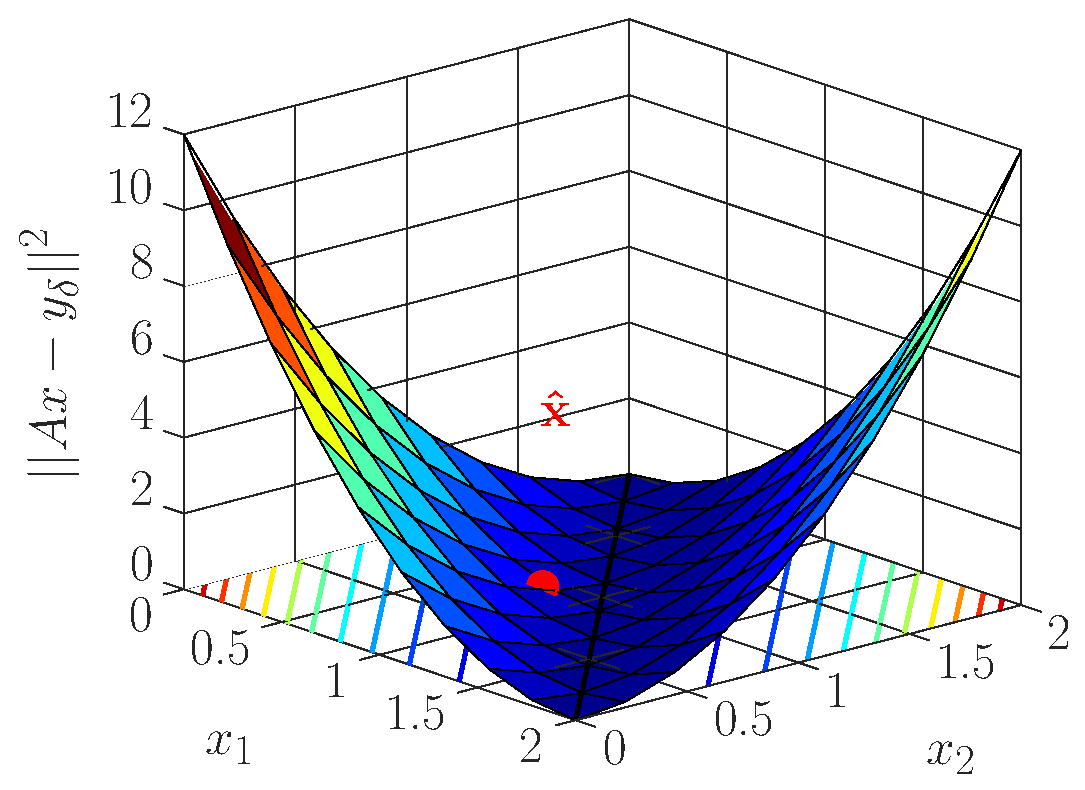
\includegraphics[width=0.98\textwidth]{chapters/notacao/mfiles/illpossed2/surfcaxyd.eps}
         \caption{Superfície $||\MATRIX{A}\VECTOR{x}-\VECTOR{y}_{\delta}||^2$ e o ponto $\VECTOR{\hat{x}}$.}
         \label{fig:ex:IllPosedMultiplaSolutions:a}
     \end{subfigure}
     \hfill
     \begin{subfigure}[b]{0.475\textwidth}
         \centering
         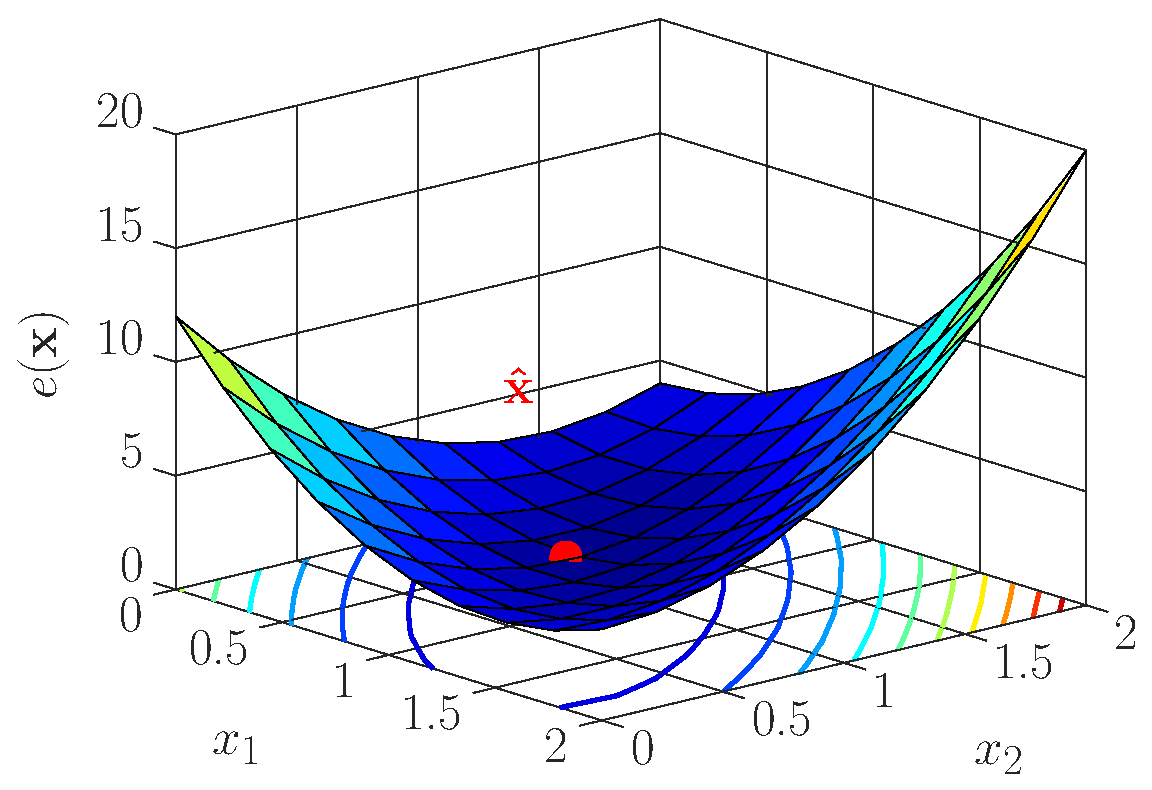
\includegraphics[width=0.98\textwidth]{chapters/notacao/mfiles/illpossed2/surfcex.eps}
         \caption{Superfície $e(\VECTOR{x})$ e o ponto $\VECTOR{\hat{x}}$. }
         \label{fig:ex:IllPosedMultiplaSolutions:b}
     \end{subfigure}
        \caption{Resposta gráfica do Exemplo \ref{ex:IllPosedMultiplaSolutions}. }
        \label{fig:ex:IllPosedMultiplaSolutions}
\end{figure}

%%%
%%%
\begin{SolutionT}[Relativa ao Exemplo \ref{ex:IllPosedMultiplaSolutions}:]
Uma forma diferente de regularizar o Exemplo \ref{ex:IllPosedMultiplaSolutions}, 
da vista na Solução \ref{sol:IllPosedMultiplaSolutions},
é usando a função de custo 
\begin{equation}\label{eq:regularization:alt}
e(\VECTOR{x})=||\MATRIX{A}\VECTOR{x}-\VECTOR{y}_{\delta}||^2+||\VECTOR{x}-\VECTOR{x}_{j}||^2,
\end{equation}
onde $\VECTOR{x}_{j}$ é um ponto escolhido por nós.
A função $e(\VECTOR{x})$ procura minimizar $||\MATRIX{A}\VECTOR{x}-\VECTOR{y}_{\delta}||^2$
e ao mesmo tempo penaliza a resposta $\VECTOR{x}$,
quanto mais longe esteja esta de $\VECTOR{x}_{j}$.
Para resolver um problema de minimização como o proposto na Eq. (\ref{eq:regularization:alt}),
usamos o Teorema \ref{theo:minAxbCAxbplusalphaxqD}, de modo que o vetor $\VECTOR{x}=\VECTOR{x}_{j+1}$ que minimiza $e(\VECTOR{x})$
é igual a
%\begin{equation}\label{eq:regularization:4b}
$
\VECTOR{x}_{j+1} =
\left[ \MATRIX{A}^{\transpose}\MATRIX{A} +\MATRIX{I}\right]^{-1}\left[ \MATRIX{A}^{\transpose} \VECTOR{y}_{\delta}+ \VECTOR{x}_{j}\right].
$
%\end{equation}

Se usamos esta equação iterativamente, desde um $\VECTOR{x}_{0}=[0\quad 0]^{\transpose}$, 
obteremos os resultados vistos na Tabela \ref{tab:IllPosedMultiplaSolution},
de modo que quando $\VECTOR{x}_{j}$ converge; é dizer, quando $\VECTOR{x}_{j+1}\approx \VECTOR{x}_{j}$,
temos uma solução;  neste caso o problema converge em $\VECTOR{x}_{7}=[1\quad 1]^{\transpose}$,
que sim cumpre o sistema $\MATRIX{A}\VECTOR{x}_{7}=\VECTOR{y}_{\delta}$.
\end{SolutionT}


\begin{table}[h!]
\centering
 \begin{tabular}{|c|c|c|c|c|c|c|c|c|} 
 \hline
 $j$ & $0$ & $1$ & $2$ & $3$ & $4$ & $5$ & $6$ & $7$ \\ \hline
 \hline
 $\VECTOR{x}_{j}$ & 0 & 0.85714 & 0.97959 & 0.99708 & 0.99958 & 0.99994 & 0.99999 & 1.00000 \\
 ~                & 0 & 0.85714 & 0.97959 & 0.99708 & 0.99958 & 0.99994 & 0.99999 & 1.00000 \\
 \hline
 \end{tabular}
\caption{Resposta iterativa na minimização da função $e(\VECTOR{x})$.}
\label{tab:IllPosedMultiplaSolution}
\end{table}



